\documentclass{article}

\usepackage{../notatka}
\usepackage[utf8]{inputenc}
\usepackage[T1]{fontenc}
\usepackage[polish]{babel}
\usepackage{array}
\usepackage{microtype}
\usepackage{makecell}
%usepackage{showframe}
\usepackage{chessboard}
%\usepackage[nomathsymbols, OT4]{polski}
\selectlanguage{polish}

%\renewcommand*\ShowFrameColor{\color{gr}}

\title{\ttfamily {\color{emp}SKOCZEK}\medskip\\ \normalsize {\color{dygresyja}rozwiązanie robocze}}
\author{{\color{tit}Łukasz Magnuszewski}}
\date{}

\begin{document}\ttfamily
\maketitle\smallskip
\begin{center}\emph{\scriptsize\color{dygresyja}spisane przez Ronię, bo tak}\end{center}

\subsection*{USUWANIE JEDNEJ PARY PÓL}
Pokażemy, że gracz drugi ma strategię wygrywającą.\smallskip\\
Pierwszy gracz usuwa dowolną parę pól: jedno czarne, drugie białe. \bigskip\\
Definiujemy graf pierwotny, gdzie krawędziami są ruchy skoczka, a wierzchołkami pola \\szachownicy.\medskip\\
Weźmy podgraf tego grafu, gdzie wierzchołki zachowujemy, a krawędzie należą do cyklu \\Hamiltona:\bigskip\\
\begin{center}
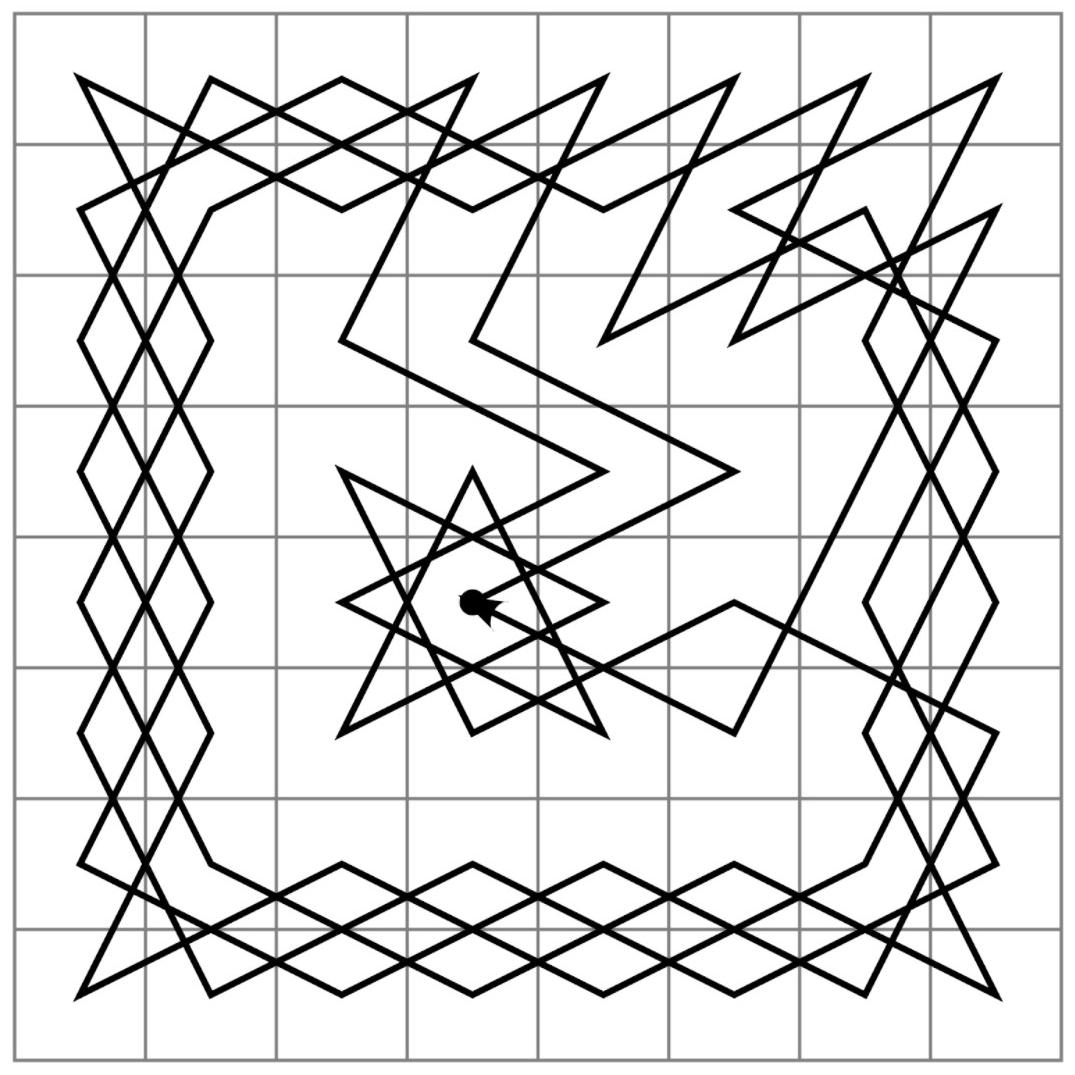
\includegraphics[scale=0.2]{podpierdalanko.png}
\end{center}\bigskip

Zauważamy, że przejście krawędzią zmienia kolor pola, gdyż każdy ruch to dwa w jednym \\kierunku i jedno w kierunku prostopadłym.\medskip\\
Jeśli usuniemy z wykresu te dwa pola, które usunął gracz pierwszy, nasz graf zostanie \\podzielony na dwie spójne składowe, każda o rozmiarze parzysty:
\pmazidlo
\draw[gray, ultra thick] (0, 0) arc (90:135:5);
\filldraw[color=acc, fill=back, ultra thick] (0, 0) circle (0.2);
\filldraw[color=tit, fill=back, ultra thick] (-1, -0.1) circle (0.2);
\filldraw[color=acc, fill=back, ultra thick] (-2, -0.4) circle (0.2);
\filldraw[color=tit, fill=back, ultra thick] (-3, -1) circle (0.2);
\node at (-3.8, -1.7) {...};
\draw[gray, ultra thick] (-3.9, -2) arc (145:190:5);
\filldraw[color=acc, fill=back, ultra thick] (-4.2, -2.5) circle (0.2);
\filldraw[color=tit, fill=back, ultra thick] (-4.6, -3.5) circle (0.2);
\filldraw[color=acc, fill=back, ultra thick] (-4.8, -4.5) circle (0.2);
\filldraw[color=tit, fill=back, ultra thick] (-4.8, -5.5) circle (0.2);

\draw[gray, ultra thick] (1, -1) arc (90:135:5);
\filldraw[color=acc, fill=back, ultra thick] (1, -1) circle (0.2);
\filldraw[color=tit, fill=back, ultra thick] (0, -1.1) circle (0.2);
\filldraw[color=acc, fill=back, ultra thick] (-1, -1.4) circle (0.2);
\filldraw[color=tit, fill=back, ultra thick] (-2, -2) circle (0.2);
\node at (-2.8, -2.7) {...};
\draw[gray, ultra thick] (-2.9, -3) arc (145:190:5);
\filldraw[color=acc, fill=back, ultra thick] (-3.2, -3.5) circle (0.2);
\filldraw[color=tit, fill=back, ultra thick] (-3.6, -4.5) circle (0.2);
\filldraw[color=acc, fill=back, ultra thick] (-3.8, -5.5) circle (0.2);
\filldraw[color=tit, fill=back, ultra thick] (-3.8, -6.5) circle (0.2);
\kmazidlo
Definiujemy bijekcję z białych (żółtych) w czarne (czerwone), a w konsekwencji bijekcę odwrotną.\medskip\\
Ponumerujmy wierzchołki od pierwszego białego końca:
\pmazidlo
\draw[gray, ultra thick] (0, 0) arc (90:135:5);
\filldraw[color=acc, fill=back, ultra thick] (0, 0) circle (0.2);
\node at (0, 0.5) {1};
\filldraw[color=tit, fill=back, ultra thick] (-1, -0.1) circle (0.2);
\node at (-1, 0.4) {2};
\filldraw[color=acc, fill=back, ultra thick] (-2, -0.4) circle (0.2);
\node at (-2, 0.1) {3};
\filldraw[color=tit, fill=back, ultra thick] (-3, -1) circle (0.2);
\node at (-3, -0.5) {4};
\node at (-3.8, -1.7) {...};
\draw[gray, ultra thick] (-3.9, -2) arc (145:190:5);
\filldraw[color=acc, fill=back, ultra thick] (-4.2, -2.5) circle (0.2);
\filldraw[color=tit, fill=back, ultra thick] (-4.6, -3.5) circle (0.2);
\filldraw[color=acc, fill=back, ultra thick] (-4.8, -4.5) circle (0.2);
\node at (-5.3, -5.5) {2n};
\filldraw[color=tit, fill=back, ultra thick] (-4.8, -5.5) circle (0.2);

\draw[gray, ultra thick] (1, -1) arc (90:135:5);
\node at (1, -0.5) {2n+1};
\filldraw[color=acc, fill=back, ultra thick] (1, -1) circle (0.2);
\node at (0, -0.6) {2n+2};
\filldraw[color=tit, fill=back, ultra thick] (0, -1.1) circle (0.2);
\filldraw[color=acc, fill=back, ultra thick] (-1, -1.4) circle (0.2);
\filldraw[color=tit, fill=back, ultra thick] (-2, -2) circle (0.2);
\node at (-2.8, -2.7) {...};
\draw[gray, ultra thick] (-2.9, -3) arc (145:190:5);
\filldraw[color=acc, fill=back, ultra thick] (-3.2, -3.5) circle (0.2);
\filldraw[color=tit, fill=back, ultra thick] (-3.6, -4.5) circle (0.2);
\filldraw[color=acc, fill=back, ultra thick] (-3.8, -5.5) circle (0.2);
\node at (-3, -6.5) {2n+2k};
\filldraw[color=tit, fill=back, ultra thick] (-3.8, -6.5) circle (0.2);
\kmazidlo

Jeśli otrzymujemy pole białe o indeksie $2p+1$, to zwracamy pole czarne o indeksie $2p+2$. Ta bijekcja ma taką własność, że jeśli przechodzimy z białego na czarne, to zawsze is-\\tnieje krawędź, która umożliwia ten ruch. Ponieważ jest to bijekcja, to możemy znaleźć odpowiednią funkcję dla skoku z czarnego na białe pole.\bigskip\\
Pokażmy, że gracz drugi wygra, czyli gracz pierwszy nie wykona ostatniego ruchu. \medskip\\
Załóżmy nie wprost, że gracz pierwszy dokona ostatni ruch na białe pole. Zdefiniowana wcześniej bijekcja zwraca nam czarne pole, na które może ruszyć się drugi gracz. \\Ponieważ mamy bijekcję z pól białych w czarne, a gracz pierwszy mógł ruszyć się tylko \\na wcześniej niewykorzystane pole, otrzymane z bijekcji czarne pole również nie zostało \\wcześniej odwiedzone.\bigskip\\
Zauważamy, że analogiczna strategia zadziała, jeśli gracz pierwszy będzie ruszał się \\na czarne pola.
\kondow

\subsection*{USUWAMY MINIMUM 2}
\begin{center}
    \setchessboard{smallboard, showmover=false}
    \def\empharea{ b7-c6 }
    \chessboard[emphstyle=\color{red}, empharea=\empharea, addpieces={na8}]
\end{center}
Pola białe (ponieważ powyżej mamy inwersję kolorów) usuwamy w dowolny sposób. Wtedy \\blokujemy już pierwszy ruch skoczkowi.\bigskip
\begin{align*}pysio&=\begin{vmatrix}x_{11}+a&&x_{21}+a&&...&&x_{n1}+a\\x_{12}&&x_{22}&&...&&x_{n1}\\...&&...&&...&&...\\x_{1n}&&x_{2n}&&...&&x_{nn}\end{vmatrix}+\begin{vmatrix}x_{11}-a&&x_{21}-a&&...&&x_{n1}-a\\x_{12}&&x_{22}&&...&&x_{n1}\\...&&...&&...&&...\\x_{1n}&&x_{2n}&&...&&x_{nn}\end{vmatrix}=\\&=\begin{vmatrix}x_{11}+a+x_{11}-a&&x_{21}+a+x_{21}-a&&...&&x_{n1}+a+x_{n1}-a\\x_{12}&&x_{22}&&...&&x_{n1}\\...&&...&&...&&...\\x_{1n}&&x_{2n}&&...&&x_{nn}\end{vmatrix}=\\&=\begin{vmatrix}2x_{11}&&2x_{21}&&...&&2x_{n1}\\x_{12}&&x_{22}&&...&&x_{n1}\\...&&...&&...&&...\\x_{1n}&&x_{2n}&&...&&x_{nn}\end{vmatrix}=\\&=\frac12\begin{vmatrix}x_{11}&&x_{21}&&...&&x_{n1}\\x_{12}&&x_{22}&&...&&x_{sn1}\\...&&...&&...&&...\\x_{1n}&&x_{2n}&&...&&x_{nn}\end{vmatrix}\end{align*}

\end{document}